\documentclass[
  11pt,
  letterpaper,
   addpoints,
   answers
  ]{exam}

\usepackage{../exercise-preamble}
\usepackage{float}
\begin{document}

\noindent
\begin{minipage}{0.47\textwidth}

\includegraphics[width=\textwidth]{../fcfm_die}
\end{minipage}
\begin{minipage}{0.53\textwidth}
\begin{center} 
\large\textbf{Fundamentos de control de sistemas} (EL4111-1) \\
\large\textbf{Clase auxiliar 10} \\
\small Prof.~Roberto Cardenas Dobson\\
\small Prof.~Aux.~Osvaldo Jimenez - Erik Sáez\\
\small Ayudantes.~Simon Arenas- Juan Pablo Baez - Francisco Garces - Sofia Ibarra\\
\end{center}
\end{minipage}

\vspace{0.5cm}
\noindent
\vspace{.85cm}

\begin{questions}
%----------------------------------------------
    \question En la tabla 1 se muestran los datos del diagrama de bode de una planta, es decir, magnitud, fase y frecuencia. Se pide encontrar un controlador con frecuencia de cruce $\omega_c$ de 14 [rad/s] y un margen de fase de 40º. El controlador debe poder asegurar C.E.E.E. para una entrada escalón.

    Para realizar esto se le pide:
    \begin{enumerate}
        \item Encontrar la fase y magnitud de la planta conociendo la frecuencia de corte.
        \item Diseñe un controlador PI que cumpla las especificaciones.
        \item Cree un nuevo controlador del tipo malla que permita cancelar un polo de la planta.
        \item ¿Cuál es el máximo retardo que puede tener la planta controlada antes que se vuelva inestable?
    \end{enumerate}
    
    \begin{table}[H]
        \centering
        \footnotesize
        \begin{tabular}{|c|c|c|}
        \hline
        \textbf{Magnitud} & \textbf{Fase} & \textbf{Frecuencia} \\
        \hline
        0,705649 & -8,91894 & 1,098541 \\
        0,70181 & -10,7241 & 1,325711 \\
        0,696331 & -12,8739 & 1,599859 \\
        0,688575 & -15,4196 & 1,930698 \\
        0,677729 & -18,41 & 2,329952 \\
        0,662813 & -21,8844 & 2,811769 \\
        0,64275 & -25,8616 & 3,393222 \\
        0,61654 & -30,3271 & 4,049415 \\
        0,583527 & -35,2205 & 4,941713 \\
        0,54372 & -40,4292 & 5,963623 \\
        0,498025 & -45,7944 & 7,196857 \\
        0,448235 & -51,132 & 8,685114 \\
        0,396708 & -56,2624 & 10,48113 \\
        0,345869 & -61,0388 & 12,64855 \\
        0,297748 & -65,3643 & 15,26418 \\
        0,253731 & -69,1928 & 18,4207 \\
        0,214537 & -72,5213 & 22,22996 \\
        0,180341 & -75,3758 & 26,82696 \\
        0,150954 & -77,7994 & 32,37458 \\
        0,125971 & -79,8422 & 39,0694 \\
        0,104898 & -81,5552 & 47,14866 \\
        0,087218 & -82,9864 & 56,89686 \\
        0,072442 & -84,1791 & 68,66488 \\
        0,060215 & -85,1714 & 82,6428 \\
        0,049878 & -85,9958 & 100 \\
        \hline
        \end{tabular}
        \caption{Datos de magnitud, fase y frecuencia}
    \end{table}
    
    
    
%----------------------------------------------
\begin{solution}
    \subsection*{Resolucion 1.1}
    Se busca encontrar la fase y magnitud de la planta considerando que el controlador con frecuencia de corte $w_{c} = 14 [rad/s]$ si observamos los valores entregados en la tabla, no se tiene un valor exacto para $w_{c}$, por lo que se debe interpolar los valores entregados:
    \begin{table}[H]
        \centering
        \footnotesize
        \begin{tabular}{|c|c|c|}
        \hline
        \textbf{Magnitud} & \textbf{Fase} & \textbf{Frecuencia} \\
        \hline
        0,345869 & -61,0388 & 12,64855 \\
        0,297748 & -65,3643 & 15,26418 \\
        \hline
        \end{tabular}
        \caption{Datos de magnitud, fase y frecuencia}
    \end{table}
    De esta manera tenemos que:
    \begin{align}
        \frac{\phi - (-61,0388)}{14-12.64855} &= \frac{-65,3643 - (-61,0388)}{15,26418 - 12,64855} \nonumber \\
        \phi &= -63,2017 \nonumber
    \end{align}
    De esta manera se obtiene el valor de fase mientras que para la magnitud , tenemos de manera similar que:
    \begin{align}
        \frac{M - 0.346}{ 14 - 12.65} = \frac{0.298 - 0.346}{15.26 - 12.65} \nonumber \\
        M = 0.322 \nonumber
    \end{align}
    Con esto se obtien tanto la ganancia como la fase de la \textbf{planta}, para la frecuencia de corte dada.
    \subsection*{Resolucion 1.2}
    Luego se busca diseñar un controlador PI que cumpla con las especificaciones del sistema, dadas por $w_{c}= 14[rad/s]$ y un margen de fase de $40^{\circ}$ y que ademas cumpla con CEEE, por lo se propone un controlador PI de la siguiente forma:
    \begin{align}
        G_{c}(j\omega) = \frac{K(jw + a)}{jw}
    \end{align}
    Se tiene que el margen actual de la planta esta dado por $\phi = -63.27$ y que el hecho de agregar un integrador produce un cambio de $90^{\circ}$ , lo que se ve representado como:
    \begin{align}
        \phi_{MF} = -63.27 - 90 = -153.27
    \end{align}
    Con lo que es posible obtener el margen de fase el cual viene dado por:
    \begin{align}
        MF = 180 + \phi_{MF} = 26.73
    \end{align}
    Es importante el destacar que adicionar el integrador producira cambios en la ganancia de la planta, por lo que se tiene que:
    \begin{align}
        M_{nueva} = \frac{0.319}{|j\omega_{c}|} = \frac{0.319}{14}  = 0.0228
    \end{align}
    (\textit{Para el calculo anterior es necesario utilizar la frecuencia de corte}). Por ultimo debemos determinar la posicion del cero, por lo que se calcula cuantos grados $\theta_{0}$ le falta para llegar a los $40^{\circ}$ esperados, por tanto:
    \begin{align}
        \text{MF}_{deseado} &= 40 = \text{MF}_{actual} + \theta_{0}\\
        \theta_{0} &= 40 - 26.73 = 13.27
    \end{align}
    Con lo que se deben agregar $13.27^{\circ}$ al margen de fase actual que lo hara el controlador PI mediante el cero (\textit{Debemos recordar que los ceros nos aportan fase, mientras que los polos restan}), por tanto:
    \begin{align}
        \tan^{-1}\left(\frac{w_{c}}{a}\right) = tan^{-1}\left(\frac{14}{a}\right) = 13.27
    \end{align}
    De esta manera se obtiene que $a = 59.36$  finalmente para determinar la ganancia del controlador se impone $|G(jw_{c})|=1$ , por lo que:
    \begin{align}
        0.023 |K| \cdot |jw_{c} + 59.36| = 0.023 \cdot | K| | j14 + 59.36| = 1
    \end{align}
    Con lo que se obtiene que $K = 0.713$ y por tanto el controlador PI vendra dado por:
    \begin{align}
        G_{c}(j\omega) = \frac{0.713(j\omega + 59.36)}{j\omega}
    \end{align}
    \subsection*{Resolucion 1.3}
    Se busca crear un controlador del tipo malla que permita cancelar un polo de la planta,por lo que primeramente se debera estimar la planta (\textit{Lo cual en plantas de mayor orden no es directo de obtener, recordemos que la motivacion de utilizar analisis en frecuencia es olvidarnos de la forma de la planta}), asumiendo que esta ultima es de primer orden, es posible estimarla cuando la fase que tiene este es aproximadamente $-45^{\circ}$, por lo que viendo la planta nos quedamos con un valor aproximado de:
    \begin{table}[H]
        \centering
        \footnotesize
        \begin{tabular}{|c|c|c|}
        \hline
        \textbf{Magnitud} & \textbf{Fase} & \textbf{Frecuencia} \\
        \hline
        0,498025 & -45,7944 & 7,196857 \\
        \hline
        \end{tabular}
        \caption{Datos de magnitud, fase y frecuencia para estimar la planta}
    \end{table}
    Recordemos que bajo lo anterior la planta en $45^{\circ}$ debera tener una forma tal que:
    \begin{align}
        G_{p}(j\omega) = K \cdot \frac{ a }{j\omega + a}
    \end{align}
    Esto se cumple unicamente cuando la planta es de primer orden y ademas se encuentra en los 45 grados.
    \begin{align}
        G_{p}(j\omega) = \frac{\hat{K}}{j\omega + 7.1968}
    \end{align}
    y para obtener el valor de $\hat{K}$ se debe considerar que su magnitud es de $0.498025$ por lo que:
    \begin{align}
        M &= \left|\frac{\hat{K}}{j\omega + 7.1968}\right| = 0.498025\\
        \hat{K} &= 5.09
    \end{align}
    Luego se repite el procedimiento anterior pero considerando que el controlador debera ser en malla, por lo tanto sera tal que:
    \begin{align}
        G_{c}(j\omega) = \frac{K ( j\omega + 7.197)}{j\omega ( j\omega + a)} 
    \end{align}
    Con lo que debemos tener en cuenta ahora que al ser un polo , este quitara fase por lo que:
    \begin{align}
        tan^{-1}\left( \frac{14}{7.197}\right) - \tan^{-1} \left( \frac{14}{a}\right) = 13.26
    \end{align}
    Con lo que a =11.947, notamos que los $13.16^{\circ}$ se mantienen dado que es la misma cantidad de fase que se necesita para el controlador PI, luego para su ganancia:
    \begin{align}
        0.023 |K| \cdot |j14 + 7.197| \cdot |14j + 11.947|^{-1} = 1
    \end{align}
    Lo que resulta un valor de K= 50.8, por lo que finalmente el controlador en malla sera:
    \begin{align}
        G_{c}(j\omega) = \frac{50.8 ( j\omega + 7.197)}{j\omega ( j\omega + 11.947)}
    \end{align}
    \subsection*{Resolucion 1.4}
    como buscamos saber cual es el maximo retardo que puede tener la planta controlada antes de que se vuelva inestable, se debe considerar que el retardo se puede modelar comse debe considerar esto courre cuando MF=0, es decir cuando:
    \begin{align}
        0 = 40 - \theta_{retardo}\\
    \end{align}
    Con lo que reemplazando la expresion conocida del retardo resultando en:
    \begin{align}
        \omega T \cdot \frac{180}{\pi} = 40 \\
        T =0.05[s]
    \end{align}

\end{solution}
%----------------------------------------------
    \question Se tienen dos plantas $G_1(s)$ y $G_2(s)$ operando en una fábrica. Dependiendo de lo que se desee producir, se deben utilizar dos modos de operación: Modo 1: Sólo está en funcionamiento $G_1(s)$. Modo 2: Se encuentran $G_1(s)$ y $G_2(s)$ trabajando en serie ($G_1(s) \cdot G_2(s)$). Se tiene la información en frecuencia de ambos modos:

    \begin{table}[H]
        \centering
        \footnotesize
        \begin{tabular}{|c|c|c|c|c|}
        \hline
        \textbf{Frecuencia} (rad/s) & \multicolumn{2}{c|}{\textbf{Modo 1}} & \multicolumn{2}{c|}{\textbf{Modo 2}} \\
        \cline{2-5}
        & \textbf{Magnitud} & \textbf{Fase (grados)} & \textbf{Magnitud} & \textbf{Fase (grados)} \\
        \hline
        0.0100 & 1.0000 & -0.5729 & 0.0049 & 89.1405 \\
        0.0137 & 0.9999 & -0.7870 & 0.0068 & 88.8193 \\
        0.0188 & 0.9998 & -1.0812 & 0.0094 & 88.3780 \\
        0.0259 & 0.9997 & -1.4853 & 0.0129 & 87.7719 \\
        0.0356 & 0.9994 & -2.0401 & 0.0177 & 86.9394 \\
        0.0489 & 0.9988 & -2.8017 & 0.0244 & 85.7965 \\
        0.0672 & 0.9977 & -3.8464 & 0.0335 & 84.2282 \\
        0.0923 & 0.9958 & -5.2772 & 0.0459 & 82.0784 \\
        0.1268 & 0.9920 & -7.2319 & 0.0628 & 79.1376 \\
        0.1743 & 0.9851 & -9.8891 & 0.0855 & 75.1291 \\
        0.2395 & 0.9725 & -13.4688 & 0.1156 & 69.7024 \\
        0.3290 & 0.9499 & -18.2129 & 0.1542 & 62.4445 \\
        0.4520 & 0.9112 & -24.3246 & 0.2008 & 52.9394 \\
        0.6210 & 0.8495 & -31.8409 & 0.2519 & 40.9099 \\
        0.8531 & 0.7607 & -40.4697 & 0.2984 & 26.4279 \\
        1.1721 & 0.6490 & -49.5302 & 0.3281 & 10.0972 \\
        1.6102 & 0.5276 & -58.1590 & 0.3308 & -6.9976 \\
        2.2122 & 0.4119 & -65.6753 & 0.3055 & -23.5595 \\
        3.0391 & 0.3126 & -71.7870 & 0.2610 & -38.4393 \\
        4.1753 & 0.2329 & -76.5312 & 0.2100 & -50.9365 \\
        5.7361 & 0.1717 & -80.1108 & 0.1621 & -60.8859 \\
        7.8804 & 0.1259 & -82.7680 & 0.1220 & -68.5274 \\
        10.826 & 0.0920 & -84.7227 & 0.0904 & -74.2562 \\
        14.873 & 0.0671 & -86.1535 & 0.0664 & -78.4951 \\
        20.433 & 0.0489 & -87.1982 & 0.0486 & -81.6080 \\
        28.072 & 0.0356 & -87.9598 & 0.0355 & -83.8466 \\
        38.566 & 0.0259 & -88.5146 & 0.0258 & -85.5460 \\
        52.983 & 0.0189 & -88.9187 & 0.0188 & -86.7569 \\
        72.789 & 0.0137 & -89.2129 & 0.0137 & -87.6390 \\
        100.000 & 0.0100 & -89.4270 & 0.0099 & -88.2812 \\
        \hline
        \end{tabular}
        \caption{Datos de frecuencia para los modos de operación de $G_1(s)$ y $G_2(s)$}
    \end{table}
    
    \begin{enumerate}
        \item[(a)] Sabiendo que la planta $G_1(s)$ es de tipo cero de primer orden y que se está operando en el modo 1, diseñe un controlador por cancelación con cero error en estado estacionario para una entrada escalón para una frecuencia de cruce de 14.873 rad/s y con un margen de fase de 45 grados. (15/50 puntos)
        
        \item[(b)] Dado el envejecimiento de la planta, aparece un retardo de 0,01 segundos. Modifique el controlador realizado en (a) para esta situación. (10/50 puntos)
        
        \item[(c)] Si se sigue operando en el modo 1 con el controlador que diseñó en (b), ¿cuál es el máximo retardo que puede tener la planta antes de que se vuelva inestable? (10/50 puntos)
        
        \item[(d)] Ahora se comienza a trabajar en Modo 2 y se necesita diseñar un nuevo controlador. Además de entregársele la tabla con la respuesta de frecuencia en el modo 2, le informan que la planta $G_2(s)$ está compuesta únicamente por un cero y un polo, pero en posiciones desconocidas (15/50 puntos por la pregunta d):
        
        \begin{itemize}
            \item Responda fundamentadamente. ¿Cuántos integradores se deberían necesitar para obtener cero error en estado estacionario cuando se utiliza la planta Modo 2?
            
            \item (Propuesto) Diseñe un controlador para operación con el Modo 2 que entregue cero error en estado estacionario para una entrada escalón, operando a una frecuencia de cruce de 3.0391 rad/s y con un margen de fase de 40 grados.
        \end{itemize}
    \end{enumerate}
    
%----------------------------------------------
\begin{solution}
\subsection*{Resolucion 2.1}
    Dado que la planta se encuentra operando solo en el modo 1, y sabiendo ademas que es de tipo cero de primer orden, se puede asumir que la planta tendra la forma:
    \begin{align}
        G_{1}(s) = K\frac{a}{s+a}
    \end{align}
    Por lo que dado que se busca realizar un controlado con cancelacion con cero error a estado estacionario para entrada escalon para una frecuencia de cruce de $14.873 [rad/s]$, se debe primeramente obtener el valor de la planta, similar a lo anterior debemos obtener su frecuencia para una fase de $45^{\circ}$, viendo la tabla se tiene:
    \begin{table}[H]
        \centering
        \footnotesize
        \begin{tabular}{|c|c|c|c|c|}
        \hline
        \textbf{Frecuencia} (rad/s) & \multicolumn{2}{c|}{\textbf{Modo 1}} & \multicolumn{2}{c|}{\textbf{Modo 2}} \\
        \cline{2-5}
        & \textbf{Magnitud} & \textbf{Fase (grados)} & \textbf{Magnitud} & \textbf{Fase (grados)} \\
        \hline
        0.8531 & 0.7607 & -40.4697 & 0.2984 & 26.4279 \\
        1.1721 & 0.6490 & -49.5302 & 0.3281 & 10.0972 \\
        \hline
        \end{tabular}
        \caption{Datos de frecuencia para los modos de operación de $G_1(s)$ y $G_2(s)$}
    \end{table}
    Por lo que se debera aproximar como:
    \begin{align}
        \frac{-49.5302 - (-45)}{1.1721 - w^{*}} = \frac{-49.5302 - (-40.4697)}{1.1721-0.8531} 
    \end{align}
Con lo que se obtiene que $w^{*}=1.10126$, luego para el valor de la ganancia de la planta se tendra que es aproximadamente $0.707$ con lo que se obtiene que :
\begin{align}
    |G_{1}(s)| = \left| k \cdot \frac{a}{s+a}\right| 
\end{align}
De esta manera reemplazando el w conocido se tendra que:
\begin{align}
    0.707 = k\frac{1.10126}{\sqrt{1.10126^{2} + 1.10126^{2}}}
\end{align}
Obteniendo un valor aproximado de $k=1$, por lo que finalmente la pltant apuede ser representada como:
\begin{align}
    G_{1}(s) = \frac{1.10126}{s+1.10126}
\end{align}
Este paso realizado es adicional, esto se puede ver de manera directa en la tabla:
\begin{table}[H]
    \centering
    \footnotesize
    \begin{tabular}{|c|c|c|c|c|}
    \hline
    \textbf{Frecuencia} (rad/s) & \multicolumn{2}{c|}{\textbf{Modo 1}} & \multicolumn{2}{c|}{\textbf{Modo 2}} \\
    \cline{2-5}
    & \textbf{Magnitud} & \textbf{Fase (grados)} & \textbf{Magnitud} & \textbf{Fase (grados)} \\
    \hline
    0.0100 & 1.0000 & -0.5729 & 0.0049 & 89.1405 \\
    \hline
    \end{tabular}
    \caption{Datos de frecuencia para los modos de operación de $G_1(s)$ y $G_2(s)$}
\end{table}
Si esta comienza con un valor de magnitud 1, luego k=1. Luego s ebusca realizar un controlador tal que cumpla:
\begin{itemize}
    \item Frecuencia de corte sea de $14.873 [rad/s]$
    \item Margen de fase de $45^{\circ}$
    \item Debe tener cero error en estado estacionario
    \item Debe cancelar un polo de la planta.
\end{itemize}
Luego el controlador propuesto, sera tal que:
\begin{align}
    G_{c}(j\omega) = K \cdot \frac{j\omega + 1.0126}{j\omega (j\omega + b)}
\end{align}
Este cumple con todo, por l oque debemos ver como obtener el valor de b y de K, para esto volvemos sobre la tabla y se obtiene el margen de la fase actual para la frecuencia de corte solicitada:
\begin{table}[H]
    \centering
    \footnotesize
    \begin{tabular}{|c|c|c|c|c|}
    \hline
    \textbf{Frecuencia} (rad/s) & \multicolumn{2}{c|}{\textbf{Modo 1}} & \multicolumn{2}{c|}{\textbf{Modo 2}} \\
    \cline{2-5}
    & \textbf{Magnitud} & \textbf{Fase (grados)} & \textbf{Magnitud} & \textbf{Fase (grados)} \\
    \hline
    14.873 & 0.0671 & -86.1535 & 0.0664 & -78.4951 \\
    \hline
    \end{tabular}
    \caption{Datos de frecuencia para los modos de operación de $G_1(s)$ y $G_2(s)$}
\end{table}
Vemos que tiene un valor de $-86.1535$, y considerando el efecto del integrador, se tendra que el MF:
\begin{align}
    \text{MF} = 180^{\circ} - 86.1535^{\circ}  - 90^{\circ} + \theta_{\text{Cero de cancelacion}}  
\end{align}
Para calcular este ultimo tenemos que:
\begin{align}
    \tan^{-1}\left(\frac{w_{c}}{1.0126}\right) = 86.1051^{\circ}
\end{align}
Con lo que el MF sera:
\begin{align}
    180 - 86.1535 - 90 + 86.1051 = 89.9516
\end{align}
y como el margen de fase deseado se busca que sea de $45^{\circ}$, se tiene que:
\begin{align}
    45 = 89.9516 - \theta_{\text{polo de cancelacion}}
\end{align}
Es importante notar que se esta realizando una resta porque este polo quita fase.
\begin{align}
    \theta_{\text{polo de cancelacion}} = 44.9516
\end{align}
Con lo que:
\begin{align}
    \tan^{-1}\left(\frac{14.873}{b}\right) = 44.9516
\end{align}
De esta manera se obtiene que $b=14.8981$, con lo que queda obtener solo la ganancia , la cual vendra dada por la condicion de modulo:
\begin{align}
    K = \left| \frac{1}{ G_{1}(j\omega) \cdot G_{c}(j\omega) }\right|_{w=w_{c}}
\end{align}
Con lo que se obtiene que K = 309.201, dando como resultado un controlador de la forma:
\begin{align}
    G_{c}(j\omega) = 309.201 \cdot \frac{j\omega + 1.0126}{j\omega (j\omega + 14.8981)}
\end{align}
\subsection*{Resolucion 2.1}
Debemos considerar ahora el efecto de un retardo de 0.01 segundos en la planta y debemos modificar el controlador, debemos tener en consideracion lo siguiente en relacion a este retardo:
\begin{itemize}
    \item No modifica la magnitud
    \item Agrega una fase de $-w_{c}T_{d}$
    \item Dependera de la frecuencia de corte
\end{itemize}
De esta manera tenemos que el retardo introducido en grados sera:
\begin{align}
    \phi_{\text{retardo}} = -14.873 \cdot 0.01 \cdot \frac{180}{\pi} = -8.516^{\circ}
\end{align}
Luego el margen de fase se vera modificado como:
\begin{align}
    \text{MF (Con retardo)} = 45^{\circ} - 8.516^{\circ} = 36.484^{\circ}
\end{align}
Luego podemos modificar el controlador ya calculado anteriormente tal que:
\begin{align}
    G_{c}(j\omega) = 309.201 \cdot \frac{j\omega + 1.0126}{j\omega (j\omega + 14.8981)} \cdot k_{m} \cdot \frac{j\omega + 14.8981}{j\omega +c}
\end{align}
Donde ahora nuestro retardo debido a la malla propuesta sera tal que:
\begin{align}
    MF_{deseado} = MF_{retardo} + \theta_{\text{Cero 14.89}} - \theta_{\text{Polo de sintonizacion}}
\end{align}
De esta manera tenemos que:
\begin{align}
    45 &= 36.4784 + 44.9516 - \theta_{\text{Polo de sintonizacion}}\\
    36.43^{\circ} = \theta_{\text{Polo de sintonizacion}}
\end{align}
Por lo tanto ya podemos obtener el valor de c de manera directa
\begin{align}
    36.43 = \tan^{-1}\left(\frac{14.8981}{c}\right)
\end{align}
Se obtiene de esta manera que $c= 20.1511$ con lo que queda obtener uicamente el valor de la ganancia $k_{m}$ por lo que utilizando la condicion de modulo se tendra:
\begin{align}
    k_{m} = \left| \frac{1}{G_{1}(j\omega) \cdot G_{c}(j\omega)}\right|_{w=w_{c}}
\end{align}
De esta manera $K_{m} =1.18973$ con lo que el controlador final sera:
\begin{align}
    G_{c}(j\omega) = 309.201 \cdot \frac{j\omega + 1.0126}{j\omega (j\omega + 14.8981)} \cdot 1.18973 \cdot \frac{j\omega + 14.8981}{j\omega + 20.1511}
\end{align} 
\subsection*{Resolucion 2.3}
Dado que se busca analizar cual sera el retador maximo tal que la planta se vuelva inestable. Sabemos de antemano que esto se cumple cuando el margen de fase es negativo, por lo que el caso limite se cumplira cuando el margen de fase sea 0, es decir:
\begin{align}
    MF_{critico} &= MF_{actual} - \theta_{\text{retardo}}\\
    0 &= 45  -w_{c} \cdot T_{d}^{*} \cdot \frac{180}{\pi} \\
\end{align}
Despejando se obtiene que $t_{d}^{*}=  0.0528 [s]$.
\subsection*{Resolucion 2.4}
Ahora debemos considerar que el sistema comienza a operar en el modo 2 , por lo que se debera diseñar un nuevo controlador, ademas se informa que la planta $G_{2}(s)$ esta compuesta por un cero y un polo, pero en posiciones desconocidas. Inicialmente se pregunta la cantidad de integradores que se necesitan para obtener cero error a estado estacionario, esto no es tan directo dado que ahora no podemos aproximar nuestra planta a primer orden, y deberemos obtener informacion en base a la tabla y recordando como se construyen los diagramas de bode:
\begin{center}
    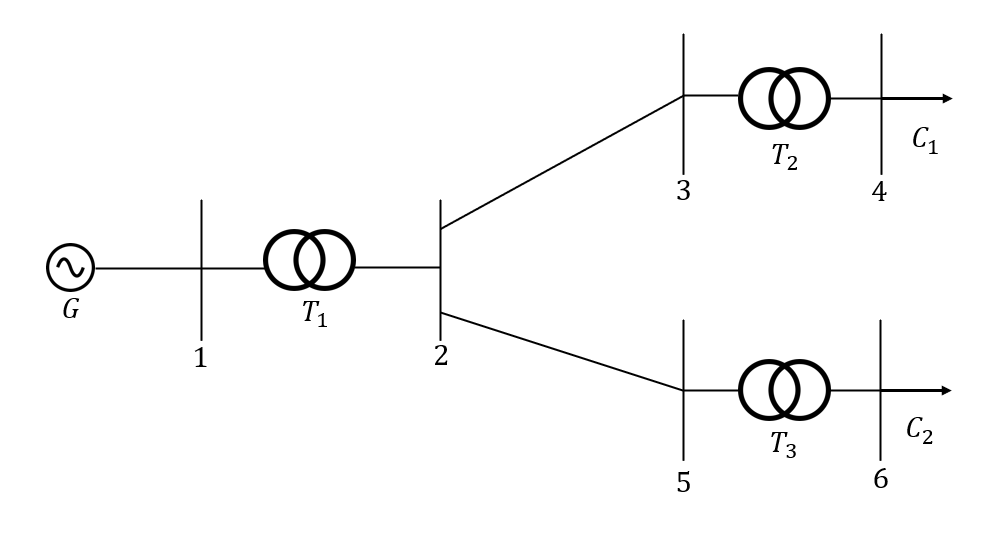
\includegraphics[width=0.7\textwidth]{Auxiliar_9_1}
    \captionof{figure}{Diagrama de Bode para un polo en el origen.}
\end{center}
\begin{center}
    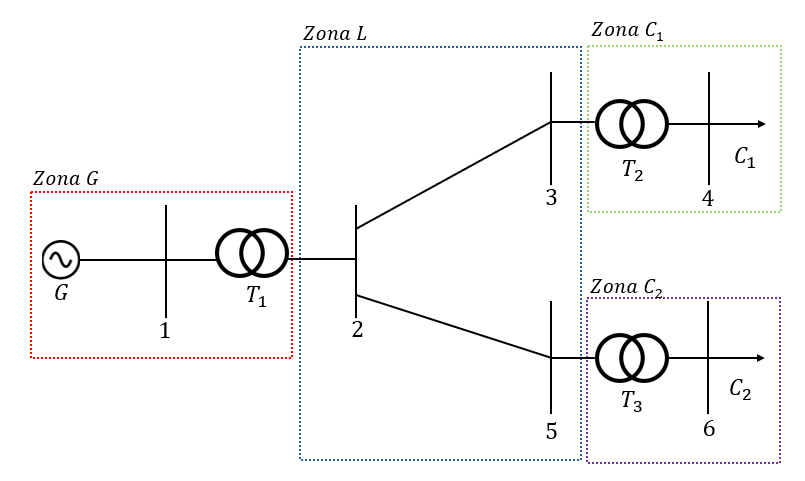
\includegraphics[width=0.7\textwidth]{Auxiliar_9_2}
    \captionof{figure}{Diagrama de Bode para un cero en el origen}
\end{center}
Volviendo sobre la tabla tenemos que:
\begin{table}[H]
    \centering
    \footnotesize
    \begin{tabular}{|c|c|c|c|c|}
    \hline
    \textbf{Frecuencia} (rad/s) & \multicolumn{2}{c|}{\textbf{Modo 1}} & \multicolumn{2}{c|}{\textbf{Modo 2}} \\
    \cline{2-5}
    & \textbf{Magnitud} & \textbf{Fase (grados)} & \textbf{Magnitud} & \textbf{Fase (grados)} \\
    \hline
    0.0100 & 1.0000 & -0.5729 & 0.0049 & 89.1405 \\
    \hline
    \end{tabular}
    \caption{Datos de frecuencia para los modos de operación de $G_1(s)$ y $G_2(s)$}
\end{table}
Vemos que comienza en $90^{\circ}$ por lo tanto corresponde un cero en el origen, por lo que es posible concluir de manera directa que para que el sistema tenga CEEE, debe tener dos integradores. 
\end{solution}
\end{questions}
%----------------------------------------------
\newpage
%%%%%%%%%%%%%%%%%%%%%%%%%%%

\end{document}